\documentclass{iSWAGArticle}

%\usepackage{lipsum}
\usepackage{amssymb}
\usepackage[dvips]{epsfig,psfrag}
\usepackage[utf8]{inputenc}

\title{In-Rank mesh optimization for URL customized promotion in SEO}
\author{\iSWAGAuthor{Stefan Duprey\\
Cdiscount\\
stefan.duprey@cdiscount.com} \and \iSWAGAuthor{Second Author\\
Second University\\
second.author@university2.com}}

\begin{document}

\maketitle

\begin{abstract}
 Web site internal mesh optimization is at the very heart of search engine optimization. 
 One prominent way to get the best web search engine visibility for our site 
 is to build the adequate internal linking to promote our naturally popular pages. 
 The definition of popular might be the transformation rate for e-commerce, 
 the traffic from logs for a common site or even a semantic quality rate for our page. 
 We here propose an algorithm to automatically compute the optimal internal mesh for our web site.
 We tackle the challenges met both at a theory and software implementation level. 
 We'll more specifically deal with big data issues for an e-commerce web site.
 \\\newline
 \indent \textbf{Keywords: }
 \\\newline
search engine, e-commerce, page rank, in rank, mesh optimization, global optimization
\end{abstract}

\section{Introduction}
We here propose an original methodology to optimize the internal mesh of Cdiscount e-commerce site.
The idea behind is to promote the most successful URLs (the most frequently viewed by users) by increasing their in-rank.  
The frequency data is obtained from logs parsing tracking software and the in rank is computed using the famous page rank iterative algorithm.  
We want to find the optimal mesh, which maximizes for all URLs the matching between their traffic and their in-rank. 
The more successful a URL is, the more in-rank we want to give him through our optimal mesh.
 \\\newline
We here detail the technical implementation of such an algorithm.
The difficulty here is three-fold:
\\
\indent
First the structure of an e-commerce is already well-defined and it is out of question to drastically change the already existing mesh.
Links are categorized regarding their incoming page type and position within that page and links can only be created within certain categories. 
So we'll have strong constraints for our mesh to comply with.
\\
\indent
Second the universe we deal with is discrete and gigantic. 
For a mesh with $N$ nodes, the number of possible meshes is $2^{N^{2}}$. 
Our objective function is non-linear and non-convex. Exhaustive optimization would be far too computationally intensive. 
We have to find a proper heuristic based global optimization algorithm to cleverly tweak through our universe.
\\
\indent
Third the actual size of our data makes the implementation of a real-world industrial use case a technologically difficult problem.
Either we implement from scratch over a cluster our algorithm dealing ourselves with concurrency and inter-processor communications,
or we try not to reinvent the wheel and plug ourselves to existing big data platform.
The double iterative nature of our algorithm (page rank computations and optimization are both naturally iterative)
makes Hadoop Map/Reduce paradigm too slow for our purpose. 
In contrast to Hadoop's two-stage disk based Map/Reduce paradigm, Spark's in-memory primitives provide the needed performance.
By allowing user programs to load data into a cluster's memory and query it repeatedly, Spark is well suited for our purpose.
We'll detail the technological implementation of a real-world use case.

\section{Algorithm}
Soit $N \in \mathbb{N}$ le nombre de noeuds de notre maillage.
 \\\newline
Soit $$\left(X_i\right)_{i \in \left\{1,...,N\right\}}$$ les sommets de notre graphe orienté.
 \\\newline
Soit $$\left(G_{ij}\right)  \in \left\{0,1\right\}^{N\times N}$$ la matrice adjacente de notre graphe orienté.
\begin{equation}
\max_{\left(G_{ij}\right)  \in \left\{0,1\right\}^{N\times N}}\left\{ \sum^{N}_{i=1} trafic\left(X_i\right)\times PR(X_i)\right\}
\end{equation}
 \\\newline
Initialisation du page rank :
\begin{equation}
\forall u \ PR\left(u\right)=\frac{1}{N}
\end{equation} 
Calcul itératif :
\begin{equation}
PR\left(u\right)= \frac{\left(1-c\right)}{N} + c \times \sum_{v \rightarrow u}\frac{PR\left(v\right)}{card\left(\left\{v\rightarrow u\right\}\right)}
\end{equation}

We here explain the genetic algorithm crossover funcTion :
 \\\newline
\textbf{\large Child from 2 parents crossover}
\begin{center}
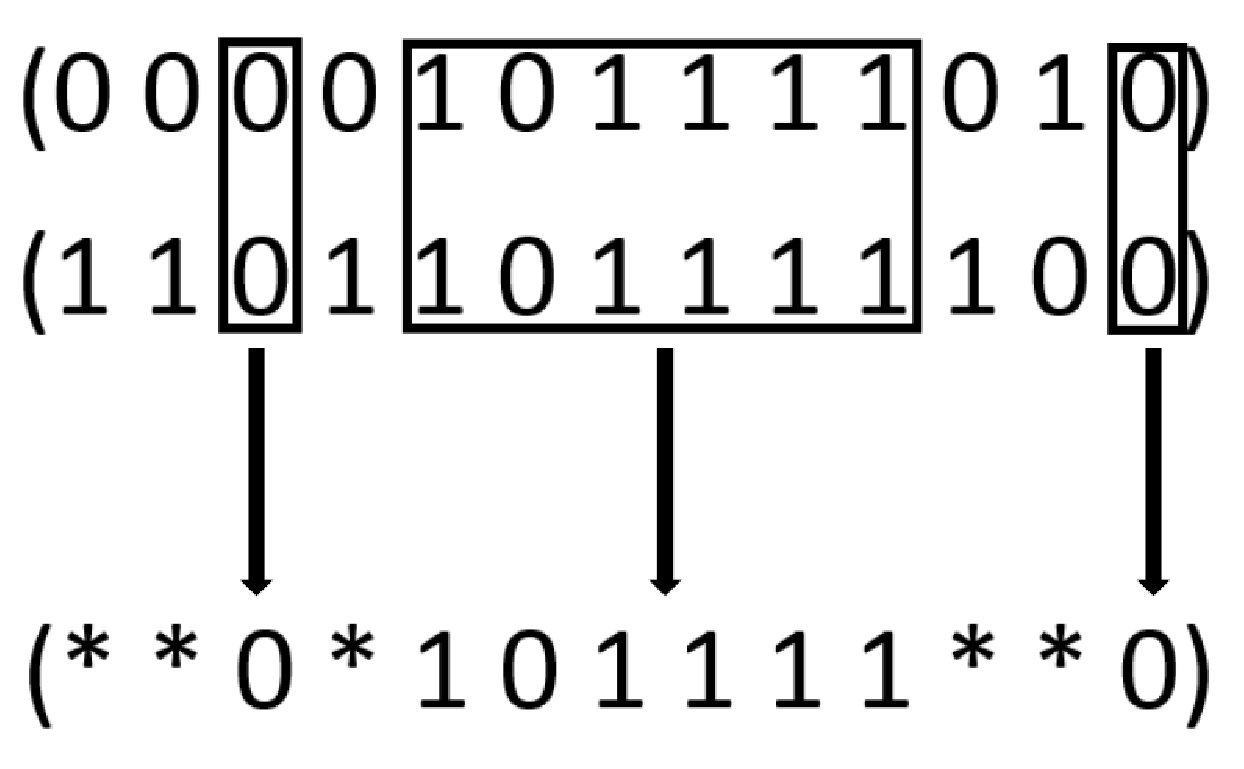
\epsfig{file=crossover.eps,height=2cm,width=4cm}
\end{center}
We here explain the genetic algorithm mutation function :
 \\\newline
\textbf{\large Mutation of an individual}
\begin{center}
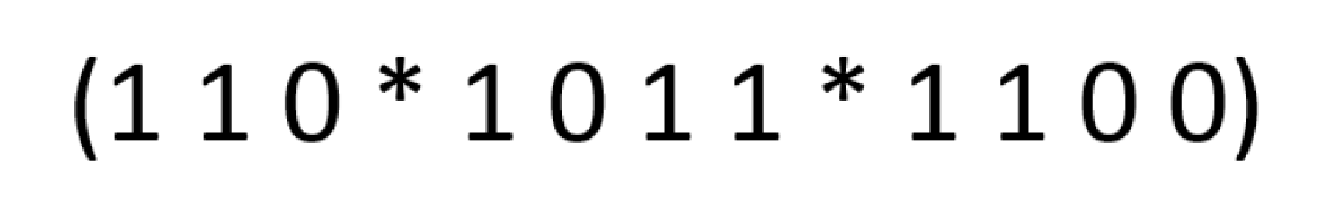
\epsfig{file=mutation.eps,height=0.4cm,width=4cm}
\end{center}
Categorization of our links :
 \\\newline
\textbf{\large Links categorization}
\begin{center}
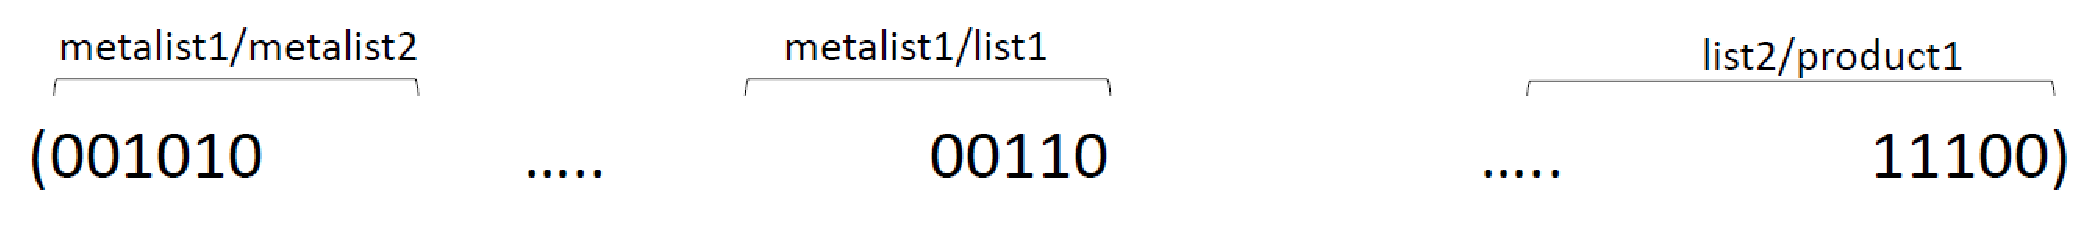
\epsfig{file=links_categorization.eps,height=1cm,width=6cm}
\end{center}

\section{Big data implementaino}
%\lipsum
%A citation example: \cite{donald1999art}.

\bibliographystyle{plain}
\bibliography{biblio}
\end{document}
